\documentclass[14pt,a4paper]{extarticle}
\usepackage[english,russian]{babel}
\usepackage{graphicx}
\usepackage{tabularx}

\usepackage{fontspec}
\setmainfont{Times New Roman}

% Margins
\usepackage[
    top=20mm,
    bottom=20mm,
    left=30mm,
    right=10mm
]{geometry}

\usepackage{setspace}
\setlength{\parindent}{15mm}  % Paragraph indent
\setstretch{1.5}  % Line height

\usepackage{titlesec}
\titleformat{\section}[hang]{\normalfont\bfseries}{\thesection}{}{}
\titlespacing{\section}{15mm}{0pt}{0pt}

\usepackage{caption}
\usepackage{subcaption}
\DeclareCaptionLabelSeparator{emdash}{ --- }
\captionsetup[figure]{name={Рисунок},labelsep=emdash}

\begin{document}
\begin{titlepage}
    \begin{center}
        {\bfseries
        МИНОБРНАУКИ РОССИИ\par
        САНКТ-ПЕТЕРБУРГСКИЙ ГОСУДАРСТВЕННЫЙ\par
        ЭЛЕКТРОТЕХНИЧЕСКИЙ УНИВЕРСИТЕТ\par
        <<ЛЭТИ>> ИМ. В.И. УЛЬЯНОВА (ЛЕНИНА)\par
        Кафедра САПР

        \vspace{0.23\textheight}
        ОТЧЁТ\par
        по практической работе №1\par
        по дисциплине <<Информационные технологии>>\par
        Тема: Знакомство с SymPy.
        \vspace{0.28\textheight}
        }
        \begin{table}[!ht]
            \begin{tabularx}{\textwidth}{p{60mm}X>{\centering\arraybackslash}p{45mm}}
                Студент гр. 4352 & \_\_\_\_\_\_\_\_\_\_\_\_\_\_\_\_\_\_\_\_ & {Даричев Е. М.} \\ [5.4mm]  % Line height
                Преподаватель    & \_\_\_\_\_\_\_\_\_\_\_\_\_\_\_\_\_\_\_\_ & {Копец Е. Е.} \\ [5.4mm]
            \end{tabularx}
        \end{table}

        Санкт-Петербург\par
        2024
    \end{center}
\end{titlepage}
\setcounter{page}{2}

% document %
\section*{Цель работы}
Познакомиться с SymPy.

\section*{Отчёт о проделанной работе}
Для работы будет использована среда программирования Visual Studio
Code с установленным набором дополнений для поддержки Python, который
включает в себя Jupiter Notebook, поэтому для работы будет использована
эта среда.

В первом задании нужно построить графики функций с помощью SymPy.
Создадим новую ячейку, в которой импортируем модуль и зададим новую
переменную. Далее создадим функцию с помощью арифметических операций и
построим её график, используя функцию $plot$. Для нахождения значений
воспользуемся функцией $f.subs$.

\begin{figure}[!ht]
    \centering
    \begin{subfigure}{.5\textwidth}
        \centering
        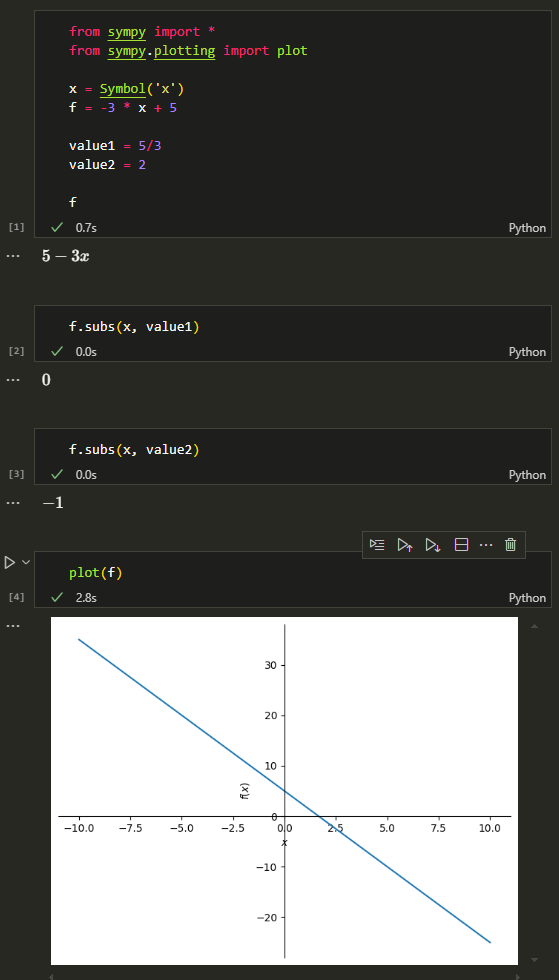
\includegraphics[width=0.9\linewidth]{figures/1.1 (1).png}
        \label{fig:1.1(1)}
    \end{subfigure}%
    \begin{subfigure}{.5\textwidth}
        \centering
        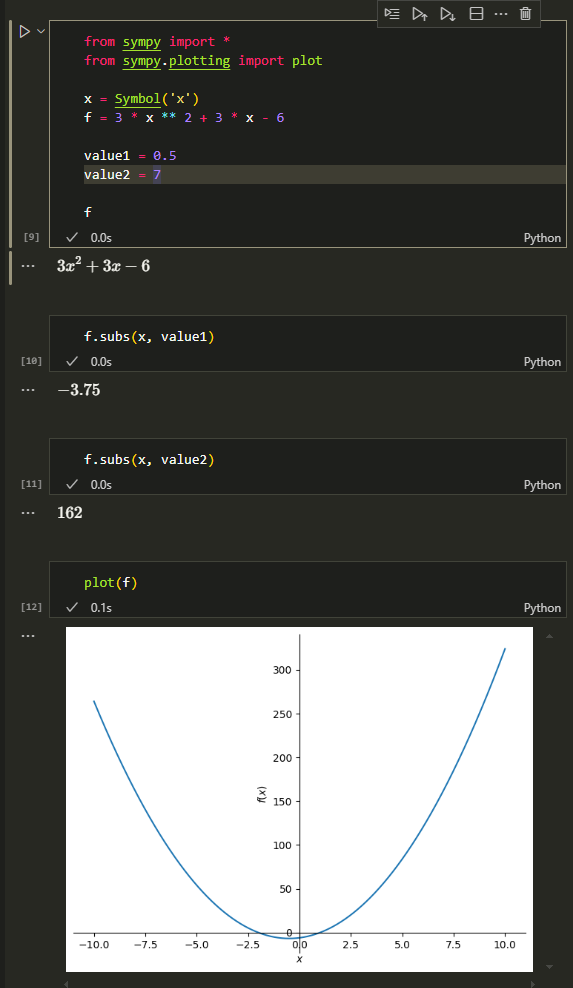
\includegraphics[width=0.9\linewidth]{figures/1.1 (2).png}
        \label{fig:1.1(2)}
    \end{subfigure}
    \caption{Задание 1.1, часть 1}
    \label{fig:1.1-part1}
\end{figure}

\begin{figure}[!ht]
    \centering
    \begin{subfigure}{.5\textwidth}
        \centering
        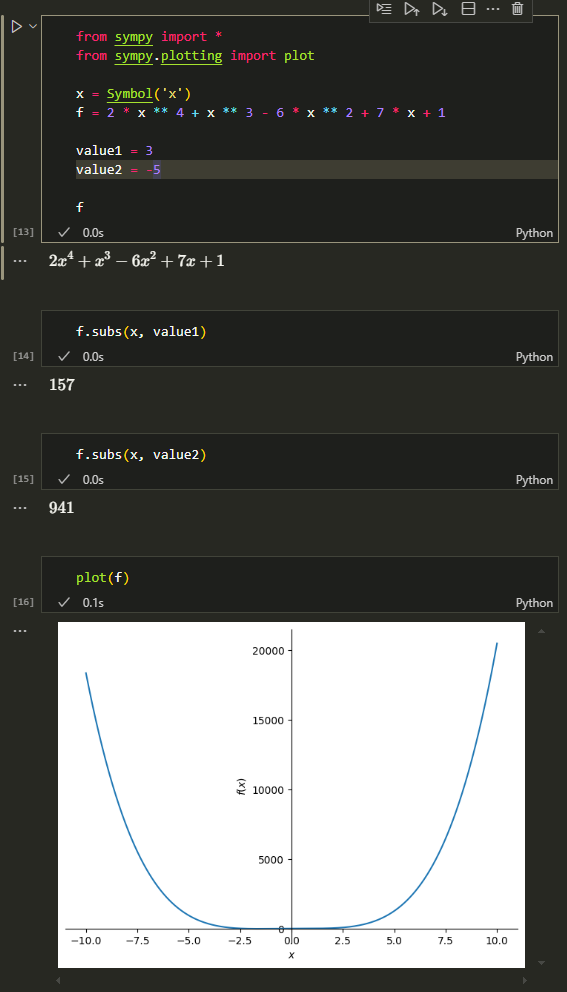
\includegraphics[width=0.9\linewidth]{figures/1.1 (3).png}
        \label{fig:1.1(3)}
    \end{subfigure}%
    \begin{subfigure}{.5\textwidth}
        \centering
        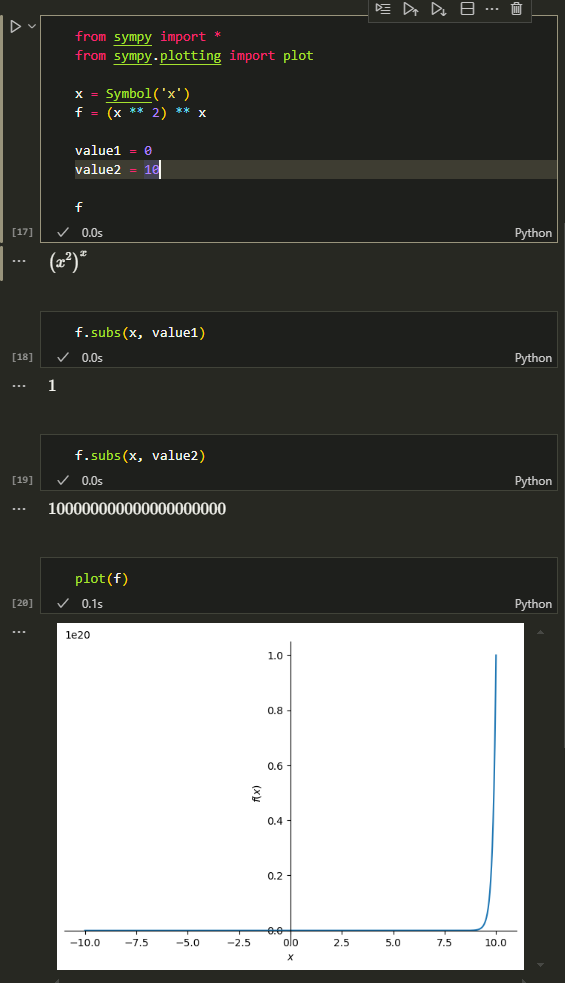
\includegraphics[width=0.9\linewidth]{figures/1.1 (4).png}
        \label{fig:1.1(4)}
    \end{subfigure}
    \caption{Задание 1.1, часть 2}
    \label{fig:1.1-part2}
\end{figure}

Во втором задании так же построим графики и проверим их на чётность
или нечётность визуально и с помощью подстановки. Для этого в отдельной
ячейке обозначим функцию с некоторыми коэффициентами и без них (рис. \ref{fig:1.2-2funcs}).
Далее будем запускать только одну из двух ячеек при построении графика и
определении вида функции.

\begin{figure}[!ht]
    \centering
    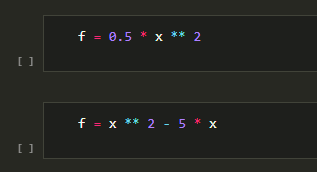
\includegraphics[width=0.5\linewidth]{figures/2 functions.png}
    \caption{Две функции в разных ячейках}
    \label{fig:1.2-2funcs}
\end{figure}

Квадратичная функция чётная, если при $f(x)=ax^2+bx+c$, $a\neq b, b=0,c=0$ (рис. \ref{fig:1.2-sq1}).
В других случаях функция имеет общий вид (рис. \ref{fig:1.2-sq2}).

\begin{figure}[!ht]
    \centering
    \begin{subfigure}{.5\textwidth}
        \centering
        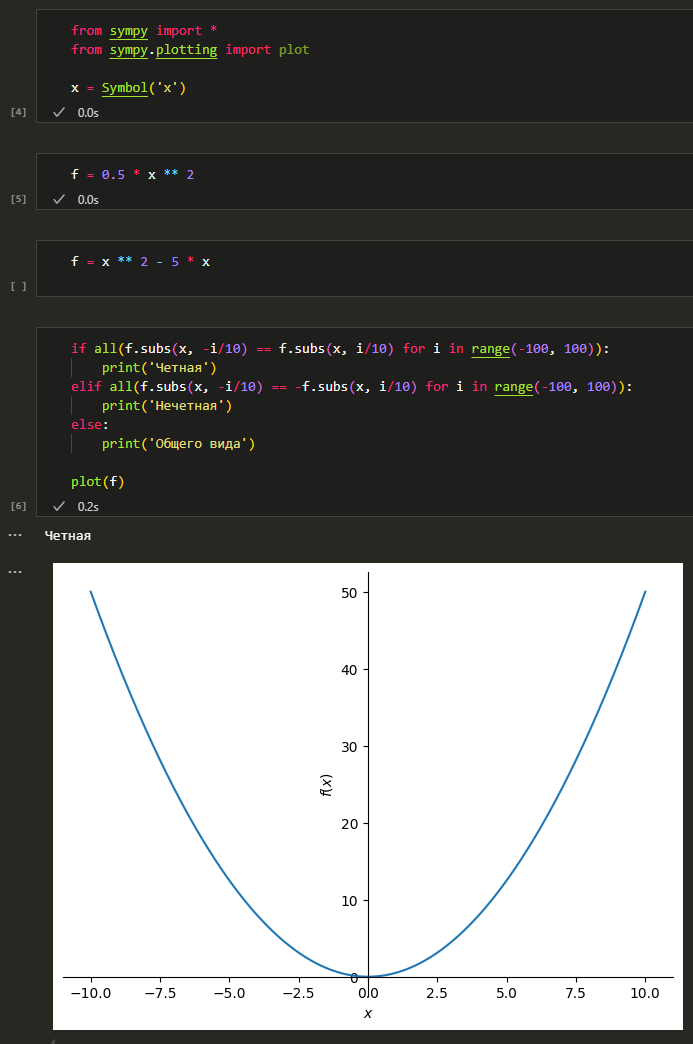
\includegraphics[width=0.9\linewidth]{figures/1.2-sq1.png}
        \caption{$a\neq b, b=0,c=0$}
        \label{fig:1.2-sq1}
    \end{subfigure}%
    \begin{subfigure}{.5\textwidth}
        \centering
        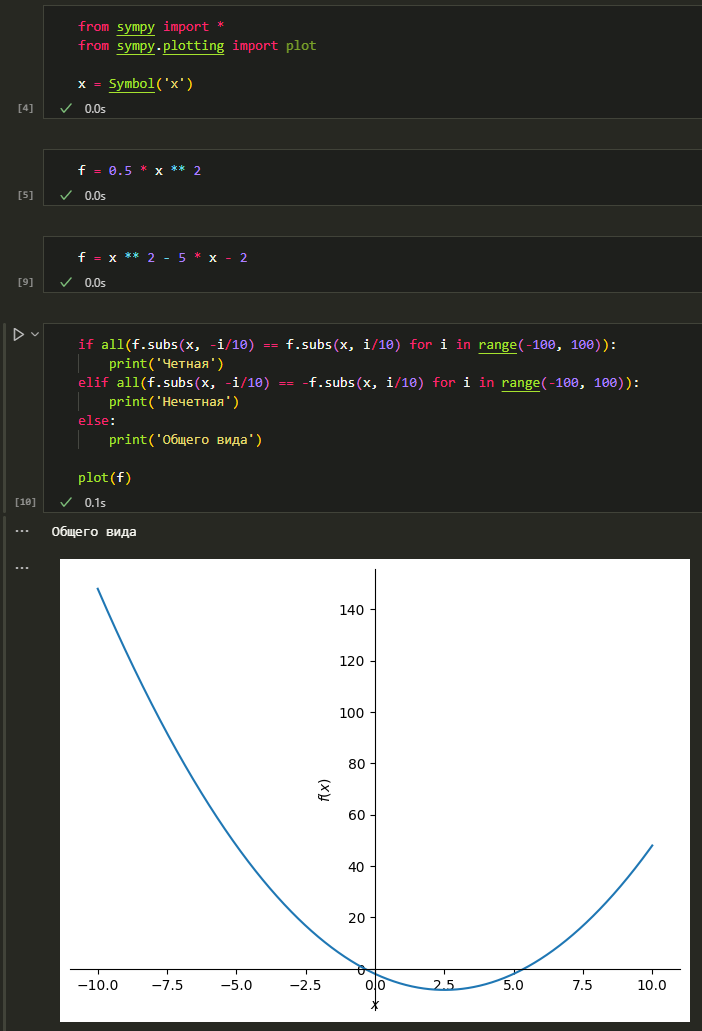
\includegraphics[width=0.9\linewidth]{figures/1.2-sq2.png}
        \caption{$a\neq b, b\neq 0,c\neq 0$}
        \label{fig:1.2-sq2}
    \end{subfigure}
    \caption{Задание 1.2, квадратичная функция}
    \label{fig:1.2-sq}
\end{figure}

Квадратичаня функция $f(x)=ax^3+bx^2+cx+d$ может быть как нечётной (рис \ref{fig:1.2-cb1}),
так и общего вида (рис \ref{fig:1.2-cb2}).
\newpage

\begin{figure}[!ht]
    \centering
    \begin{subfigure}{.5\textwidth}
        \centering
        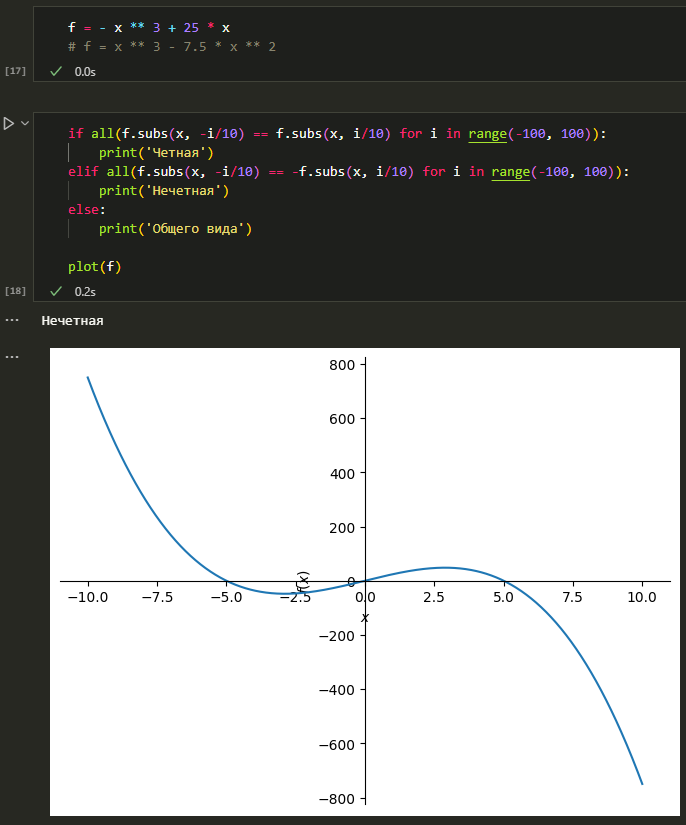
\includegraphics[width=0.9\linewidth]{figures/1.2-cb1.png}
        \caption{$a=-1,b=0,c=25,d=0$}
        \label{fig:1.2-cb1}
    \end{subfigure}%
    \begin{subfigure}{.5\textwidth}
        \centering
        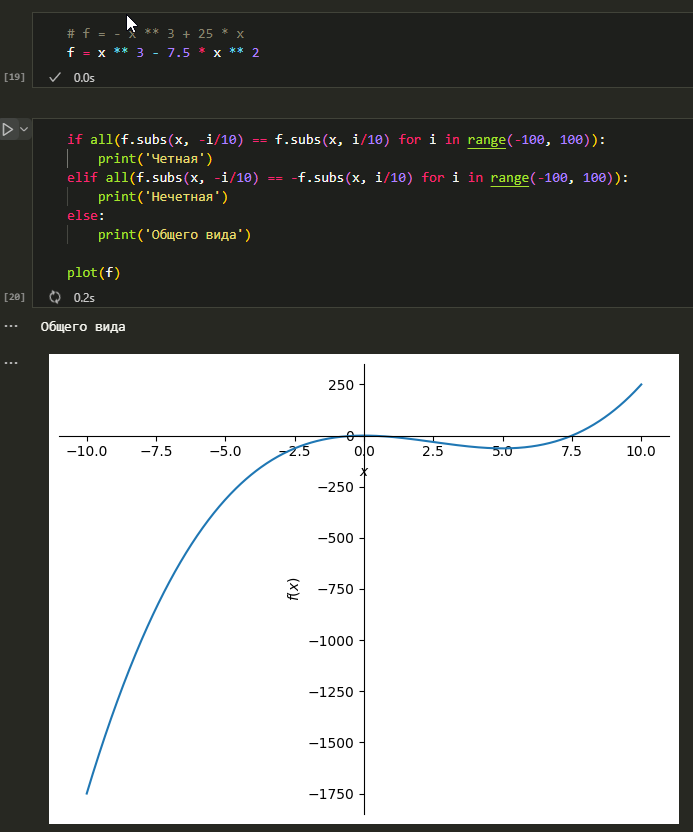
\includegraphics[width=0.9\linewidth]{figures/1.2-cb2.png}
        \caption{$a=-1,b=0,c=-7,5,d=0$}
        \label{fig:1.2-cb2}
    \end{subfigure}
    \caption{Задание 1.2, квадратичная функция}
    \label{fig:1.2-cb}
\end{figure}

Экспоненциальную функцию $f(x)=e^x$ зададим с помощью константы $E$, импортированной из модуля.
Показательную функцию $f(x)=a ^ x$ зададим так же, как и в предыдущем задании.

\begin{figure}[!ht]
    \centering
    \begin{subfigure}{.5\textwidth}
        \centering
        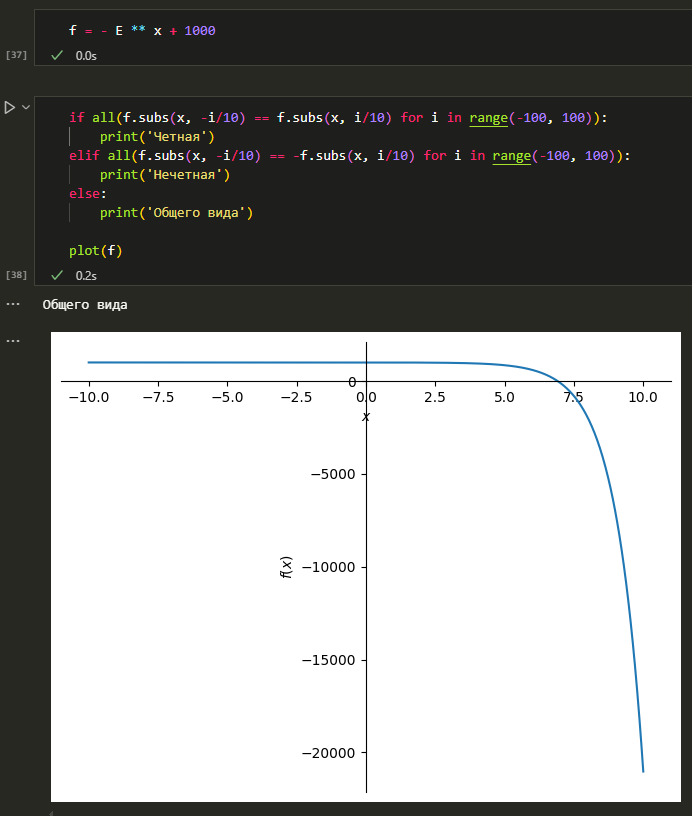
\includegraphics[width=0.9\linewidth]{figures/1.2-exp.png}
    \end{subfigure}%
    \begin{subfigure}{.5\textwidth}
        \centering
        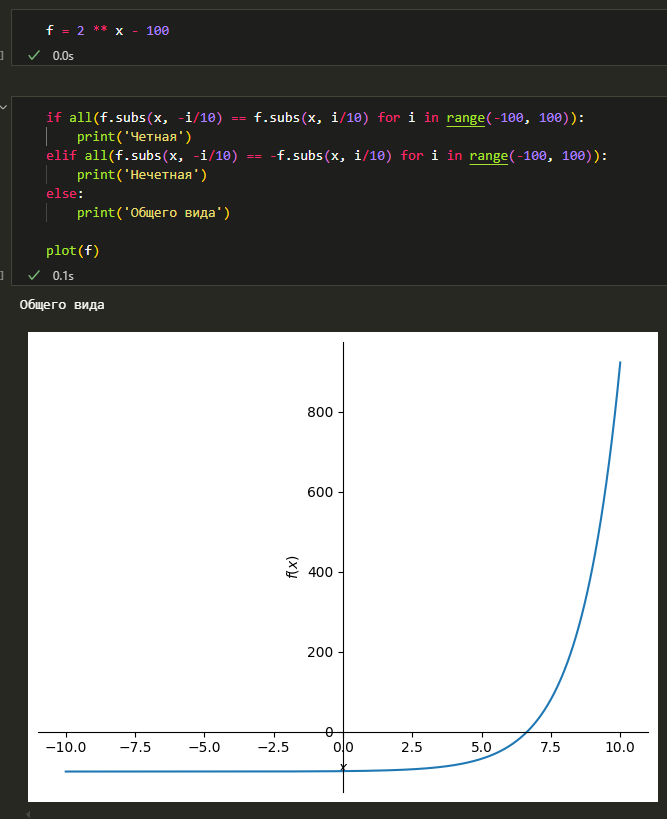
\includegraphics[width=0.9\linewidth]{figures/1.2-a.png}
    \end{subfigure}
    \caption{Задание 1.2, экспоненциальная и показательная функции}
    \label{fig:1.2-exp}
\end{figure}

В третьем задании будем искать нули функции с помощью функции $solve$
и промежутки с помощью функции  $solve\_univariate\_inequality$.

\begin{figure}[!ht]
    \centering
    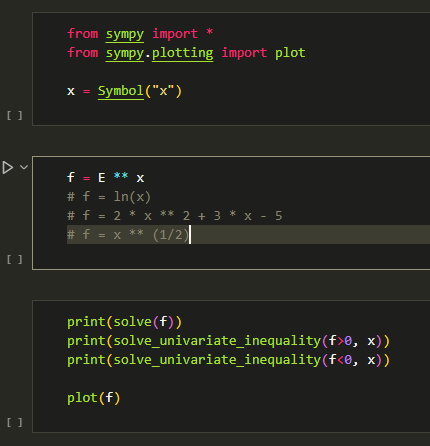
\includegraphics[width=0.5\linewidth]{figures/1.3 code.png}
    \caption{Задание 1.3, код решения}
    \label{fig:1.3-code}
\end{figure}

Функция $f(x)=e^x$ положительна на всём промежутке и не имеет нулей (рис. \ref{fig:1.3 exp}).
Функция $f(x)=ln(x)$ имеет один ноль, больше нуля от 1 до бесконечности
и меньше нуля от нуля до единицы (рис. \ref{fig:1.3 ln})
Функция $f(x)=2x^2+3x-5$ имеет два нуля, два положительных и один
отрицательный промежуток (рис. \ref{fig:1.3 sq}).
Функция $f(x)=\sqrt x$ имеет единственный ноль в $x=0$ и положительна на всём промежутке.

\newpage
\begin{figure}[!ht]
    \begin{subfigure}{0.5\textwidth}
        \centering
        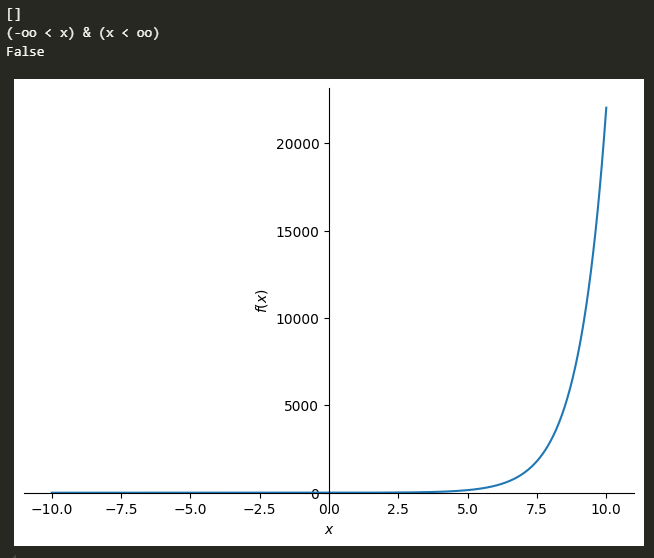
\includegraphics[width=0.9\linewidth]{figures/1.3-1.png}
        \caption{Экспоненциальная функция}
        \label{fig:1.3 exp}
    \end{subfigure}
    \begin{subfigure}{0.5\textwidth}
        \centering
        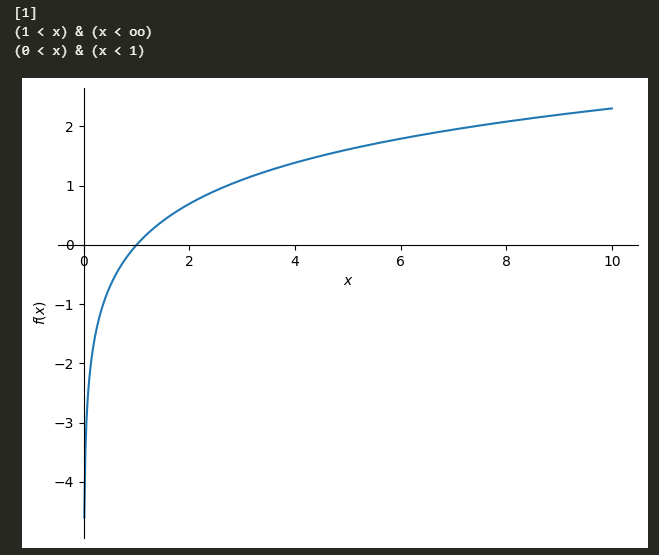
\includegraphics[width=0.9\linewidth]{figures/1.3 ln.png}
        \caption{Логарифмическая функция}
        \label{fig:1.3 ln}
    \end{subfigure}%
    \begin{subfigure}{0.5\textwidth}
        \centering
        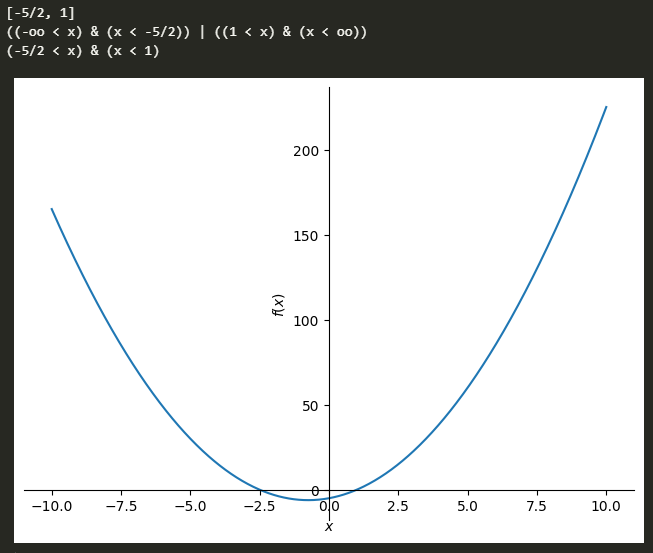
\includegraphics[width=0.9\linewidth]{figures/1.3 sq.png}
        \caption{Квадратичная парабола}
        \label{fig:1.3 sq}
    \end{subfigure}%
    \begin{subfigure}{0.5\textwidth}
        \centering
        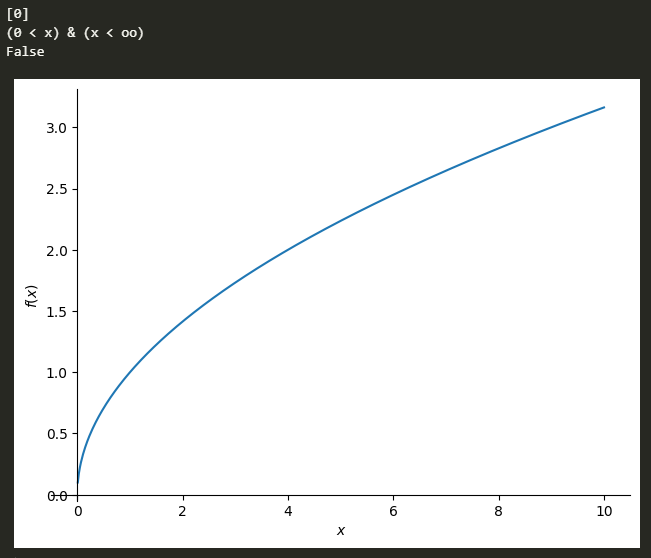
\includegraphics[width=0.9\linewidth]{figures/1.3 sqrt.png}
        \caption{Функция квадратного корня}
        \label{fig:1.3 sqrt}
    \end{subfigure}
    \caption{Задание 1.3, результат работы кода и графики}
    \label{fig:1.3}
\end{figure}

\section*{Вывод}
В ходе выполнения работы я познакомился с основами расчётов и построения графики
с помощью библиотеки SymPy.

\end{document}